\section{Approach Overview}
\label{untegriscreen:sec:systemDesign}

%We start by providing the general idea of visual supervision of user input; then discuss challenges to be addressed successfully to ensure that interactions with the remote server match user's intentions.


%\subsection{Approach Overview}
%\label{sec:systemDesign:overallApproach}


We start by providing the general idea of visual supervision of user input, depicted in Figure~\ref{fig:systemModel}.
A visual supervision system consists of 3 main components: (i) the web form and its code, running on an untrusted local client; (ii) the trusted remote \server with a dedicated component; and (iii) an app running on the user's secondary camera-equipped device, previously enrolled to the remote service. The general flow of the user's interaction with a visual supervision system is the following:

\begin{enumerate}
  \item[\one] The user enters the data through the form running in the untrusted client's browser.

  \item[\two] The visual supervision app extracts the data that is input by the user by performing optical character recognition (OCR) of the client screen in order to generate a visual \textit{\POI}.

  \item[\three] The browser transfers the user's input over a \https channel to the remote server.

  \item[\four] The visual supervision app transfers the generated \POI to the remote server over a dedicated \tls channel between the secondary device and the remote server.

  \item[\five] Upon receiving data from both the browser and the secondary device, the server matches the data from two inputs.
  If the two inputs match exactly, the web server accepts the input; otherwise, it rejects it.
\end{enumerate}



\begin{figure}[t]
    \centering
    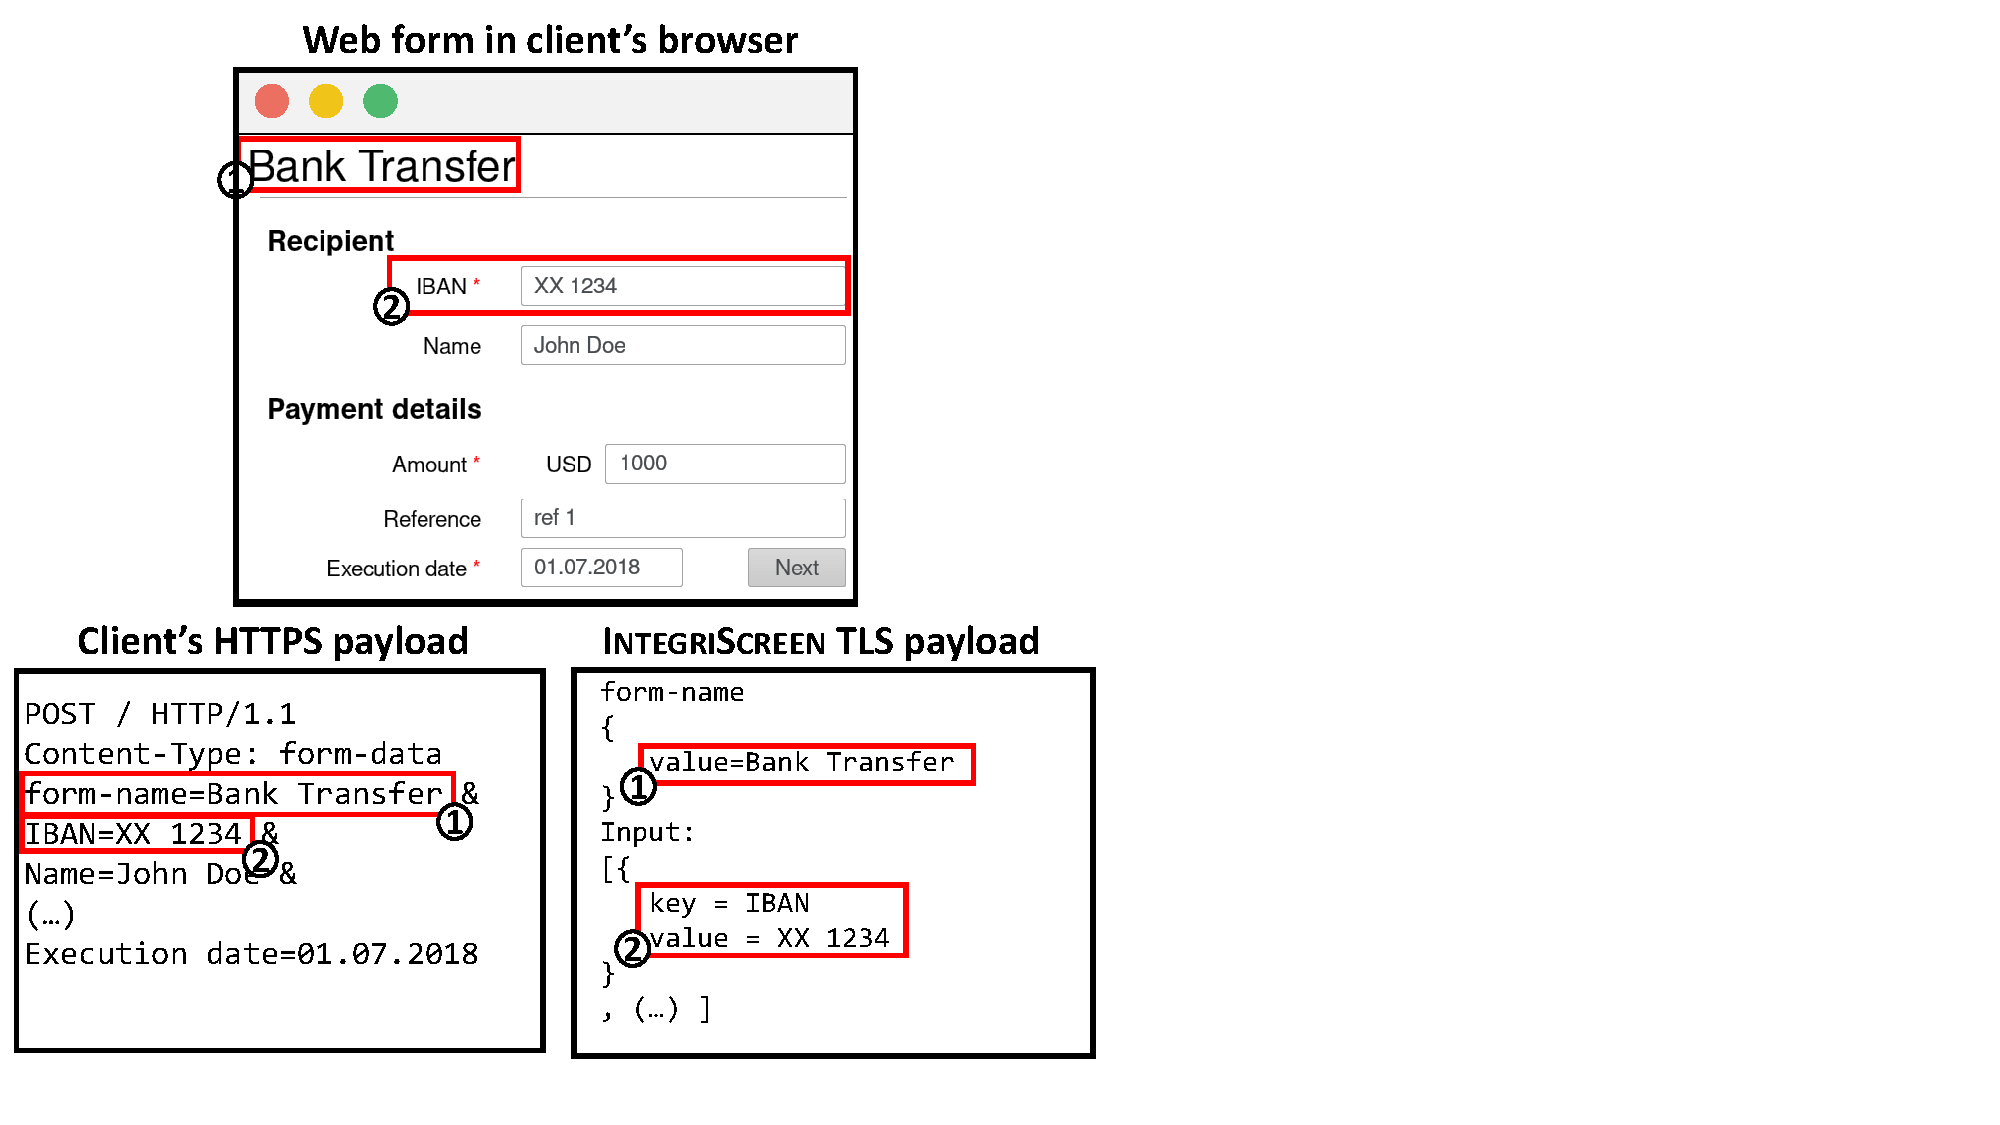
\includegraphics[trim={0 1cm 15cm 0},clip,width=0.9\linewidth]{chapters/IntegriScreen/img/inputMatching.pdf}
\caption{\textbf{\name input data matching.}
        The server receives data (e.g., \one and \two) from two channels: (i) the \https channel from the client, and (ii) the TLS channel from the \name mobile app.}
    \label{fig:traceMatching}
\end{figure}



% \myparagraph{Security of the approach}
A visual supervision provides new opportunities to defend against the attacks discussed in Section~\ref{sec:intro}.
Even after compromising the client and obtaining the victim's authentication credentials, the adversary can neither generate new requests, nor covertly modify the data before submitting.
This is prevented by the server, which would reject the requests due to not receiving a matching \POI.


\subsection{Challenges}
\label{sec:systemDesign:challenger}

Following are the challenges and possible attacks to be addressed to ensure that all received requests truly correspond with the user's intended input:

\begin{enumerate}

\item \textbf{UI manipulation attacks}
The attacker could lunch more sophisticated attack targeting the semantics of the UI. For example, the attacker can swap labels of two text fields or change the unit of an input in the label. This would result in a drastic change in input as described in existing work such as IntegriKey~\cite{integrikey}. Hence, preserving the integrity of the UI is a crucial challenge. Note that these attacks would be successful even if the user re-types his inputs into a special device that generates a TAN (transaction authorization number) code.


\item \textbf{On-screen data modification attacks}
%So far, there was no explicit discussion of the moment at which mobile app captures the data shown on the screen.
If the data shown on the client's screen are correctly sent to the remote server, the integrity of user input is not necessarily guaranteed if data extraction happens only when the form is submitted.
Despite the user entering the intended data, an adversary can subsequently modify the content of the screen in such a way that the user does not notice the change, the \app records it, and the server thus receives the same maliciously modified data from both channels. For example, in the web form shown in Figure~\ref{fig:systemModel}, the attacker can modify the IBAN number while the user sets the transaction amount or the execution date. 

 

\item \textbf{Feasibility and easy integration}
Given that detecting computer screens in images is an open research question~\cite{detectingScreens}, the recognition of form elements on screen is a challenge also. Hence, building a system that requires \emph{minimal changes to the user interface}, while at the same time maintaining the performance and achieving security guarantees against the adversarial client system poses a significant challenge. For instance, doing OCR on the whole screen degrades the performance ($<0.5$ fps) and has low classification accuracy. Camera position is an important factor to steadily track and supervise the form completion, however, another line of research in AR/VR focuses to address this issue~\cite{objectDetectionMobicom19, objectDetectionNIPS15, objectDetectionBD18}.

\end{enumerate}

\subsection{Design Goals}
\label{sec:systemDesign:designgolaks}

\myparagraph{Design Goals} Given the challenges mentioned above, a successful user input supervision to extract user intent should:

\begin{enumerate}
	\item Authenticate inputs that users make through compromised clients, i.e., ensure that the adversary cannot manipulate existing remote requests successfully.

	\item Ensure that users are not manipulated into entering and submitting data that they would not submit in the absence of the adversary.

	\item Require minimal added interaction in the absence of attacks: do not require users to input or explicitly verify any data except on the client device.
\end{enumerate}